\documentclass[convert={density=300,size=1080x800,outext=.png}]{standalone}
\usepackage{tikz}

\thispagestyle{empty}

\begin{document}
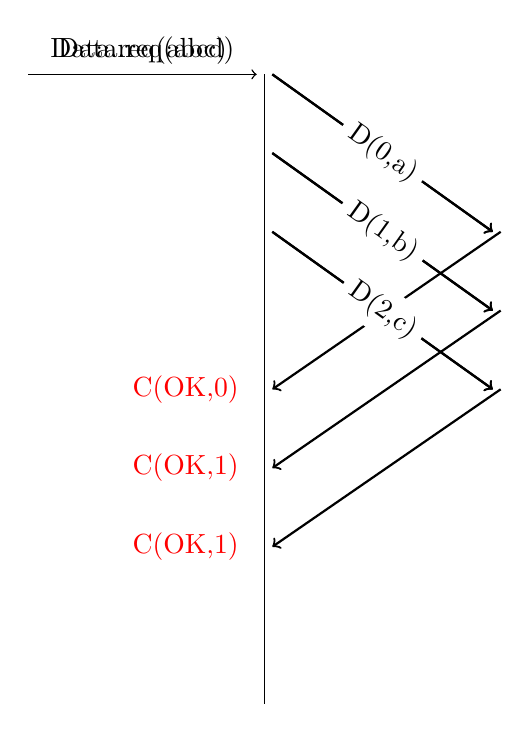
\begin{tikzpicture}
 % vertical lines 
                \draw (4,0) -- (4,-8);
                %window of 3 
                % data request 
                \draw [->] (1,0) --  node [above] {Data.req(abcd)} (3.9,0);
                \draw [->, thick] (7,-3) -- (4.1,-5) ;
                \node at (3,-5) (cok1) [color=red] {C(OK,1)};
                %data at the end 
                \draw [->, thick] (4.1,0) -- (6.9,-2) node [midway, sloped, fill=white] {D(0,a)};
                \draw [->, thick] (4.1,-1) -- (6.9,-3) node [midway, sloped, fill=white] {D(1,b)};
                \draw [->, thick] (4.1,-2) -- (6.9,-4) node [midway, sloped, fill=white] {D(2,c)};               % vertical lines 
                \draw (4,0) -- (4,-8);
                %window of 3 
                % data request 
                \draw [->] (1,0) --  node [above] {Data.req(abc)} (3.9,0);
                %
                \draw [->, thick] (7,-2) -- (4.1,-4);
                \node at (3,-4) (cok0) [color=red] {C(OK,0)};
                \draw [->, thick] (7,-4) -- (4.1,-6);
                \node at (3,-6) (cok2) [color=red] {C(OK,1)};
                %data at the end 
                \draw [->, thick] (4.1,0) -- (6.9,-2) node [midway, sloped, fill=white] {D(0,a)};
                \draw [->, thick] (4.1,-1) -- (6.9,-3) node [midway, sloped, fill=white] {D(1,b)};
                \draw [->, thick] (4.1,-2) -- (6.9,-4) node [midway, sloped, fill=white] {D(2,c)};
\end{tikzpicture}
\end{document}
